\tikzstyle{every node}=[font=\scriptsize]
\tikzset{
  >=stealth',
  fmt/.style  = { draw, fill=yamabuki, black, rounded corners, text centered},
  suc/.style = { ->, thick, shorten <=-2pt, shorten >=-2pt},
  sim/.style = {ruri, ->, decorate, decoration={snake, pre length=2pt, post length=2pt, amplitude=2pt}, >=stealth, thick, shorten <=-2pt, shorten >=-2pt}
}
\def\historyofmarkup{%
  \begin{tikzpicture}[remember picture,overlay]
  \node[fmt] (text90) at (0.75,0.25) {Text90};
  \node[fmt, right=0.3cm of text90] (runoff) {RUNOFF};
  \node[fmt, right=0.5cm of runoff] (troff) {TRoff};
  \node[right=0.3cm of runoff] (dummy0) {};
  \node[fmt, below=0.05cm of dummy0] (eqn) {EQN};

  \node[right=0.3cm of text90] (dummy1) {};
  \node[fmt, below=0.5cm of dummy1] (tex) {\TeX};

  \node[fmt, below=0.5cm of tex] (scribe) {Scribe};
  \node[right=2cm of scribe] (dummy2) {};
  \node[fmt, above=0.25cm of dummy2] (latex) {\LaTeX};

  \node[fmt, below=0.5cm of scribe] (gml) {IBM GML};
  \node[fmt, right=0.25cm of gml] (sgml) {SGML};
  \node[right=1cm of sgml] (dummy3) {};
  \node[fmt, above=0.25cm of dummy3] (html) {HTML};
  \node[fmt, below=-0.25cm of dummy3] (xml) {XML};
  \node[fmt, right=1.5cm of xml] (asciidoc) {AsciiDoc};

  \node[fmt, below=3cm of sgml] (ewb) {EWB};
  \node[fmt, right=4.5cm of ewb] (review) {Re:VIEW};

  \node[below=5cm of text90] (dummy4) {};
  \node[fmt, right=0cm of dummy4, text width=3em] (web) {文芸的プログラミング};
  \node[fmt, right=0.25cm of web, text width=3.5em] (swd) {ソフトウェアドキュメント};
  \node[fmt, right=0.25cm of swd] (pod) {pod};
  \node[fmt, below=0.25cm of xml] (setext) {setext};
  \node[fmt, right=0.5cm of pod] (rest) {reST};
  \node[fmt, right=0.5cm of rest] (md) {Markdown};
  \node[fmt, below=0.25cm of rest] (rd) {RD};

  \node[fmt, right=0.5cm of html] (wiki) {Wiki記法};
  \node[right=3.5cm of html] (dummy5) {};
  \node[fmt, above=0.75cm of dummy5] (htmlbook) {HTMLBook};

  \node[right=of md] (dummy6) {};
  \node[above=0cm of dummy6] (dummy7) {};
  \node[below=0cm of dummy6] (dummy8) {};

  \draw[suc] (text90) to (runoff);
  \draw[suc] (runoff) to (troff);
  \draw[suc] (gml) to (sgml);
  \draw[suc] (sgml) to (xml);
  \draw[sim] (sgml) to (html);
  \draw[suc] (scribe) to (sgml);
  \draw[suc] (scribe) to (html);
  \draw[suc] (scribe) to (latex);
  \draw[sim] (html) to (wiki);
  \draw[sim] (html) to (htmlbook.west);
  \draw[sim] (xml) to (asciidoc);
  \draw[suc, <->] (eqn) to (tex);
  \draw[suc] (tex) to (latex);
  \draw[suc] (web) to (swd);
  \draw[suc] (swd) to (pod);
  \draw[suc] (pod) to (rest);
  \draw[suc] (pod) to (rd);
%  \draw[sim] (sgml) to (setext);
  \draw[suc] (setext) to (rest);
  \draw[suc] (setext) to (md);
  \draw[sim] (html) to (md);
  \draw[suc] (rest) to (md);
  \draw[suc] (ewb) to (review);
  \draw[suc] (rd) to (review);

  \draw[suc] (md) to (dummy6);
  \draw[suc] (md) to (dummy7);
  \draw[suc] (md) to (dummy8);
  \end{tikzpicture}
}

\begin{frame}[t]{\inhibitglue 入力フォーマットの起源と変遷}
  \sffamily
  \historyofmarkup
\end{frame}

\begin{frame}[t]{\inhibitglue 入力フォーマットの起源と変遷$^{\ \text{[要出典]}}$}
  \sffamily
  \historyofmarkup
\end{frame}

\begin{frame}[t]{\inhibitglue 入力フォーマットの起源と変遷$^{\ \text{[要出典]}}$}
  \sffamily
  \historyofmarkup
  \begin{tikzpicture}[remember picture,overlay]
  \node[notice={(0.75,0.15)}, font=\small, text width=4cm, text centered] at (2,-1.5) {ターゲット向けの出力指示をコマンドとしてテキスト中に挿入};
  \node[notice={(2,0.15)}, font=\small, text width=4cm, text centered] at (2,-1.5) {ターゲット向けの出力指示をコマンドとしてテキスト中に挿入};
  \node[notice={(4,0.15)}, font=\small, text width=4cm, text centered] at (2,-1.5) {ターゲット向けの出力指示をコマンドとしてテキスト中に挿入};
  \pause;
  \node[notice={(3.5,-6.25)}, font=\small, text width=2cm, minimum height=1cm, text centered] at (4,-5) {これも?};
  \end{tikzpicture}

\end{frame}

\begin{frame}[t]{\inhibitglue 入力フォーマットの起源と変遷$^{\ \text{[要出典]}}$}
  \sffamily
  \historyofmarkup
  \begin{tikzpicture}[remember picture,overlay]
  \node[notice={(2.25,-2.85)}, font=\small, text width=3cm, minimum height=2cm, text centered] at (4.75,-2.5) {ターゲットによらない高レベルな記述を意識};
  \node[notice={(3.75,-0.35)}, font=\small, text width=3cm, minimum height=2cm, text centered] at (4.75,-2.5) {ターゲットによらない高レベルな記述を意識};
  \end{tikzpicture}

\end{frame}

\begin{frame}[t]{\inhibitglue 入力フォーマットの起源と変遷$^{\ \text{[要出典]}}$}
  \sffamily
  \historyofmarkup
  \begin{tikzpicture}[remember picture,overlay]
  \node[notice={(1.65,-2)}, font=\small, text width=3cm, minimum height=2cm, text centered] at (1.5,-3.5) {構造と表現の分離という概念の発明};
  \end{tikzpicture}

\end{frame}

\begin{frame}[t]{\inhibitglue 入力フォーマットの起源と変遷$^{\ \text{[要出典]}}$}
  \sffamily
  \historyofmarkup
  \begin{tikzpicture}[remember picture,overlay]
    \draw[thick] (7,0.55) rectangle (11.25,-0.25);
    \draw[sim] (7.5,0.15) to (8.5,0.15);
    \node[text width=2cm,black,font=\scriptsize] at (10,0.15) {特定ターゲット向けに簡素化};
    \pause;
    \node[notice={(10.25,-0.15)}, font=\small, text width=2.5cm, minimum height=1.5cm, text centered] at (10,-1.65) {先祖返り?};

  \end{tikzpicture}

\end{frame}


\begin{frame}[t]{\inhibitglue 入力フォーマットの指向性}
  \sffamily
  \noindent\hspace*{-2em}
  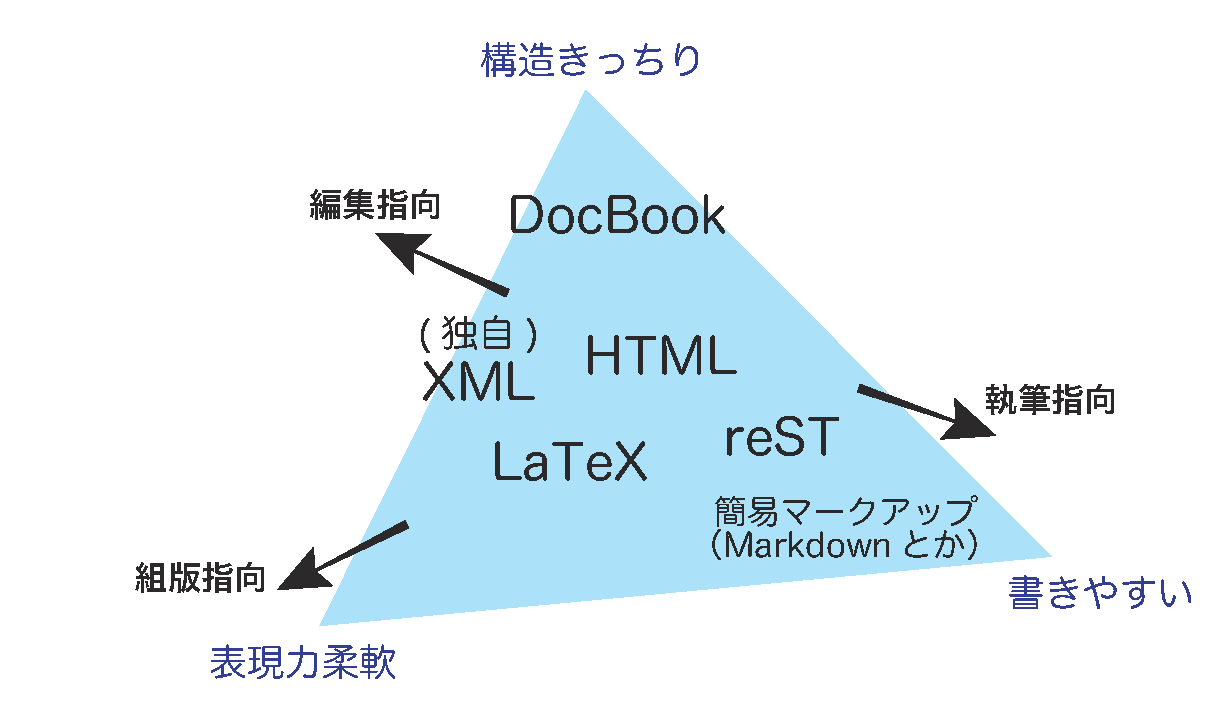
\includegraphics[width=\textwidth]{images/docsystems1.pdf}

\end{frame}



